\subsection{Корпус тонкого клиента}

Как указано выше, микрокомпьютер Raspberry Pi поставляется без корпуса. Соответственно,
требуется разработать конструкцию для защиты платы от внешних воздействий. Конструкция
не должна препятствовать охлаждению системы, иначе возникнут проблемы с
производительностью.

Так как плата Raspberry Pi является достаточно популярной, для нее существуют различные
варианты корпусов, как официальные, так и модели от сторонних производителей. Для
разработки нужно проанализировать имеющиеся варианты.

\begin{enumerate}
    \item Корпус Waveshare Electronics 11619 \cite{ref:case_oval}. Корпус выполнен из
        черного пластика, состоит из двух пластин и задней стенки с перфорацией.
        Пластины скрепляются саморезами, 4 шт. Задняя стенка устанавливается в пазы.
        Стоимость: 630 рублей.

        Корпус изображен на рисунке~\ref{pic:case_oval}.
        Так как приток холодного воздуха к SoC не обеспечен, есть опасность перегрева
        чипа. Данный корпус использовался на этапе тестирования сетевой части изделия.

    \item Корпус Waveshare Electronics 11655 \cite{ref:case_off}. Официальный корпус от
        Raspberry Pi Foundation. Корпус выполнен из пяти пластиковых частей со съемными
        крышкой и боковыми частями белого цвета.  Обеспечивает быстрый доступ к портам
        камеры и дисплея, а так же разъему расширения HAT. Предусмотрена съемная боковая
        часть для удобного доступа к 40-контактному порту GPIO.
        Стоимость: 810 рублей.

        Корпус изображен на рисунке~\ref{pic:case_oval}.
        Корпус обеспечивает охлаждение чипа только при снятии верхней крышки, при этом
        отсутствует защита платы от механических повреждений. Также возможность снятия
        боковых частей является излишней.
        
    \item Корпус Seeed Studio 114990129 \cite{ref:case_fan}.
        Корпус из акрила толщиной 3мм, с вентилятором. Вентилятор должен быть подключен
        к портам GPIO для питания.
        Стоимость: 1020 рублей.

        Корпус изображен на рисунке~\ref{pic:case_fan}.
        Вентилятор малого диаметра (30~мм) увеличивает уровень шума изделия. При его
        снятии в крышке остается полость, оставляющая SoC незащищенным.
\end{enumerate}

Все рассмотренные варианты не удовлетворяют требованиям, поставленным в задаче на
разработку. Для решения конструктивных проблем будет разработан корпус для изделия,
обеспечивающий пассивное охлаждение.

\begin{figure}[h]
    \center
    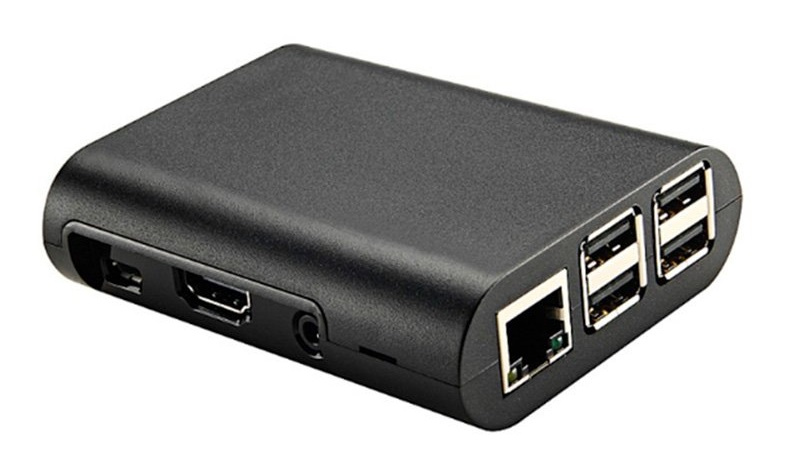
\includegraphics[height=9cm]{case_oval}
    \caption{Внешний вид корпуса Waveshare Electronics 11619}
    \label{pic:case_oval}
\end{figure}

\begin{figure}[h]
    \center
    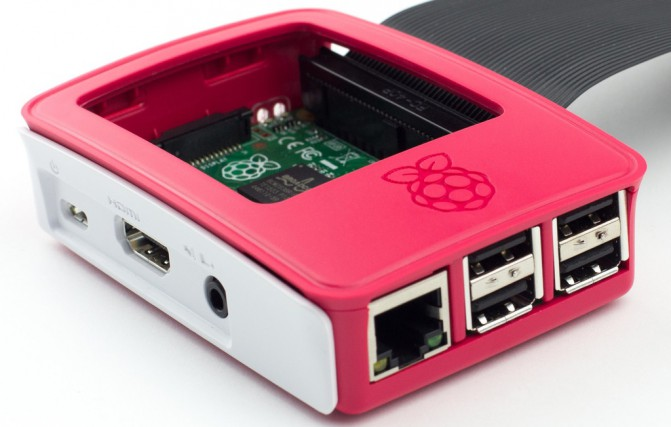
\includegraphics[height=9cm]{case_off}
    \caption{Внешний вид корпуса Waveshare Electronics 11655 с установленной платой
    Raspberry Pi}
    \label{pic:case_off}
\end{figure}

\begin{figure}[h]
    \center
    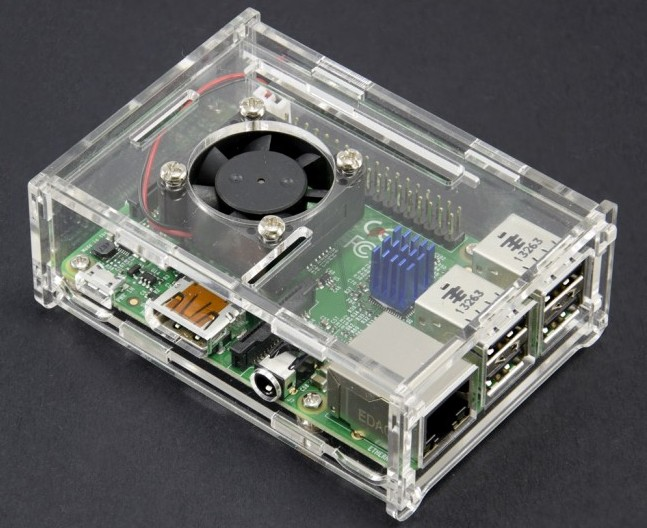
\includegraphics[height=9cm]{case_fan}
    \caption{Внешний вид корпуса Seeed Studio 114990129}
    \label{pic:case_fan}
\end{figure}
